\section{Introduction}

%{\color{red} Notes from call with Badrish:
%Move 3 goals to end of intro, rewrite into short narrative form instead of
%list. In ideas list: expand partitioned point to be clearer. Combine async
%clients with global cut; bring in word sessions. Kick hw accel to end where
%we say session batching works well with cloud hw accel offerings for low-cost
%networking/dispatching. Finally, say sessions play key rol ein parallel data
%migration.}

% XXX This could be stronger if it gave a time window and had a citation.
Millions of sensors, mobile applications, users, and machines now
continuously generate billions of events.
%
These events are processed by streaming
engines~\cite{spark-streaming,trill} and ingested and aggregated
by state management systems (Figure~\ref{fig:pipeline}).
%
Real-time queries are issued against this ingested data to train and
update models for prediction, to analyze user behavior, or to generate
device crash reports, etc.
%
Hence, these state management systems are a focal point for massive numbers of
events and queries over aggregated information about them.

Recently, this has led to specialized KVSs that can
ingest and index these events at high rates -- 100 million operations (Mops) per second (s) per machine -- by
exploiting many-core hardware~\cite{faster,anna}.
%
These systems are efficient if events are generated on the same machine as
the KVS, but, in practice, events need to be aggregated from a wide
and distributed set of data sources.
%
Hence, fast indexing schemes alone only solve part of the problem.
%
To be practical and cost-effective, a complete system for aggregating these
events must ingest events over the network, must scale across machines as
well as cores, and must be elastic (by provisioning and reconfiguring over
inexpensive cloud resources as workloads change).

\begin{figure}[t]
\centering
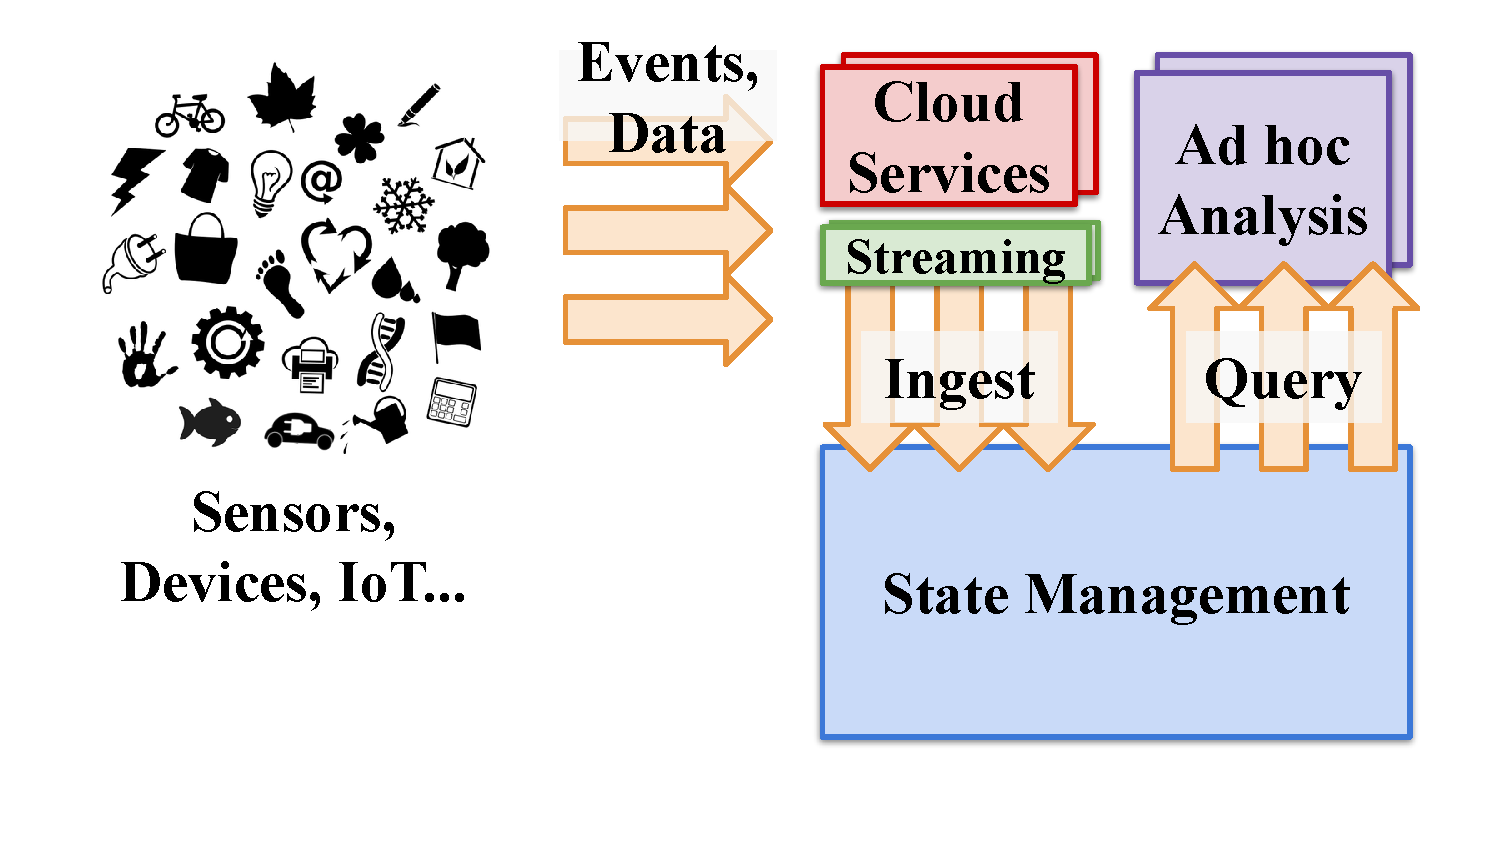
\includegraphics[width=0.93\columnwidth]{figures/pipeline.pdf}
\caption{
A typical data processing pipeline. Services receive and
process raw events and data. A state management system ingests processed
events and data, and serves offline queries against them.}
\label{fig:pipeline}
\end{figure}


The only existing KVSs that provide similar
performance~\cite{mica,flexnic,floem,kvdirect} rely on application-specific
hardware acceleration, making them impossible to deploy on today's cloud
platforms.
%
Furthermore, these systems only store data in DRAM, and they do not scale across
machines; adding support to do so without cutting into normal-case performance
is not straightforward.
%
For example, many of them statically partition records across cores to
eliminate cross-core synchronization.
%
This optimizes normal-case performance, but it makes concurrent
operations like migration and scale out impossible; transferring record data
and ownership between machines and cores requires a stop-the-world approach
due to these systems' lack of fine-grained synchronization.

Achieving this level of performance while fulfilling all of these
requirements on commodity cloud platforms requires solving two key challenges
simultaneously.
%
First, workloads change over time and cloud VMs fail, so systems must tolerate
failure and reconfiguration.
%
Doing this without hurting normal-case performance at 100~Mops/s is hard, since
even a single extra server-side cache miss to check key ownership or
reconfiguration status would cut throughput by tens-of-millions of operations
per second.
%
Second, the high CPU cost of processing incoming network
packets easily dominates in these workloads,
especially since, historically, cloud networking stacks have not been designed
for high data rates and high efficiency.
%
We show this is changing; by careful design of each server's data path, cloud
applications can exploit transparent hardware acceleration and offloading
offered by cloud providers to process more than 100~Mops/s per cloud virtual
machine (VM).

We present \emph{Shadowfax}, a new distributed KVS that transparently
spans DRAM, SSDs, and cloud blob storage while serving 130~Mops/s/VM over
commodity Azure VMs~\cite{azure} using conventional Linux TCP.
%
Beyond high single-VM performance, its unique approach to
distributed reconfiguration avoids any server-side key ownership checks
and any cross-core coordination during
normal operation and data migration both in its indexing and network interactions.
%
Hence,
it can shift load in 17~s to improve cluster throughput by
10~Mops/s
with little disruption.
%
Compared to the state-of-the-art, it has 8$\times{}$ better throughput (than
Seastar+memcached~\cite{seastar}) and scales out 6$\times{}$ faster (than
Rocksteady~\cite{rocksteady}).

In this paper, we describe and evaluate three key pieces of Shadowfax that
eliminate coordination throughout the client- and server-side by eliminating
cross-request and cross-core coordination:
%
\begin{description}
\item[Low-cost Coordination via Global Cuts:]
% All of the major components of Shadowfax including indexing, request
% dispatching, durability, checkpointing/recovery, and migration center
% around a key mechanism: asynchronous \emph{global cuts}~\cite{faster,cpr,scalog}.
%
In contrast to totally-ordered or stop-the-world approaches used by most
systems, cores in Shadowfax avoid stalling to synchronize with one another, even when
triggering complex operations like scale-out, which require
defining clear before/after points in time among concurrent operations.
%
Instead, each core participating in these operations -- both at clients and
servers -- independently decides a point in an \emph{asynchronous global
cut} that defines a boundary between operation sequences in these complex operations.
%
In this paper, we extend asynchronous cuts from cores within one process~\cite{faster,cpr} to servers
and clients in a cluster, and we show how they coordinate server
and client threads (through partitioned sessions) by detailing
their role in Shadowfax's low-coordination data migration and
reconfiguration protocol.

%for complex operations like checkpointing, recovery, and
%reconfiguration, Shadowfax makes pervasive use of asynchronous \emph{global
%cuts}.
%
%In this paper, we mainly focus on how global cuts help coordinate both server
%and client threads through partitioned sessions by focusing in detail on
%their role in Shadowfax's low-coordination data migration and
%reconfiguration protocol.
%%
%To maintain high throughput when moving ownership of records between two
%server VMs, Shadowfax takes a \emph{global cut} across
%server threads, and propagates it independently to client threads.
%%
%This allows the index to be shared under normal operation
%while avoiding serial bottlenecks during scale out.

\item[End-to-end Asynchronous Clients:]
All requests from a client on one machine to Shadowfax are asynchronous with
respect to one another all the way throughout Shadowfax's client- and
server-side network submission/completion paths and servers' indexing and
(SSD and cloud storage) I/O paths.
%
This avoids all client- and server-side stalls due to head-of-line
blocking, ensuring that clients can always continue to generate requests and
servers can always continue to process them.
%
In turn, clients naturally batch requests, improving server-side high
throughput especially under high load.
%
This batching also suits hardware accelerated network offloads available in
cloud platforms today further lowering CPU load and improving throughput.
%
Hence, despite batching, requests complete in less than 40~\us to 1.3~ms at
more than 120~Mops/s/VM, depending on which transport and hardware
acceleration is chosen.
%
% Our experiments show that this combination works well for both linux TCP
% and two-sided RDMA.

\item[Partitioned Sessions, Shared Data:]
Asynchronous requests eliminate blocking {\em between requests} within a client, but
maintaining high throughput also requires minimizing coordination
costs {\em between cores} at clients and servers.
%
Instead of partitioning data among cores to avoid synchronization on record
accesses~\cite{hstore,voltdb,mica,seastar}, Shadowfax partitions network
sessions across cores; its lock-free hash index and log-structured record heap
are shared among all cores.
%
This risks contention when some records are hot and frequently
mutated, but this is more than offset by the fact that no software-level
inter-core request forwarding or routing is needed within server VMs.

\end{description}

The rest of the paper is organized as follows. We provide background on the FASTER
key-value store and its use of epochs within a machine (\S\ref{sec:fasterkv}). Next,
we overview Shadowfax's design, including partitioned client
sessions with global cuts and how they enable
reconfiguration~(\S\ref{sec:design}). We then provide details on our parallel
non-blocking migration and scale-out techniques~(\S\ref{sec:scale-out}).
%
\iffalse
In the remainder of this paper, we describe how the key synchronization
mechanisms at the core of \faster{}'s design (\S\ref{sec:epochs}) naturally led
to Shadowfax's sessions that extend global cuts over the network
(\S\ref{sec:sessions}). We describe how this enables Shadowfax to perform the
same over the network as with a local \faster{}
instance~(\S\ref{sec:eval:clients}), and we describe how they enable
reconfiguration~(\S\ref{sec:ownership}) and parallel data
migration~(\S\ref{sec:scale-out}). We also describe how Shadowfax does this
while supporting larger-than-memory datasets that span SSD and cloud blob
storage.
\fi
%
Next, we evaluate Shadowfax in detail against other state-of-the-art shared-nothing
approaches~(\S\ref{sec:eval}), showing that by eliminating record ownership
checks and cross-core communication for routing requests it improves
per-machine throughput by 8.5$\times$ on commodity cloud VMs.
%
We also show it retains high throughput during migrations and scaled it
to a
cluster that ingests and indexes 400~Mops/s in total,
%
which, to the best of our knowledge, is the highest
reported throughput for a distributed KVS till date. We finally cover
related work~(\S\ref{sec:related}) and conclude the paper~(\S\ref{sec:conclude}).
